\documentclass[a4paper,11pt]{article}
%Premeable
	%Chinese
	\usepackage[UTF8,fontset=fandol]{ctex}
	\usepackage{xeCJK}
	\usepackage[datesep=/]{datetime2}
	\DeclareTextFontCommand{\textbf}{\sffamily}
%Presenting
	\usepackage[table]{xcolor}
	\usepackage{graphicx}
	\usepackage[font={sf}]{caption}
	\usepackage[above]{placeins}
	\usepackage{float,wrapfig}
	\usepackage{tabularx,array,booktabs,multirow,bigstrut}
	\newcolumntype{C}[1]{>{\hsize=#1\hsize%
		\centering\arraybackslash}X}
	\newcommand{\minitab}[2][l]{%
		\begin{tabular}{#1}#2\end{tabular}}
%MathSetting
	\let\latexointop\ointop
	\usepackage{amsmath,bm,amssymb,esint,extarrows}
	\usepackage{upgreek,textcomp,mathrsfs}
	\usepackage[only,sslash]{stmaryrd}
	\usepackage{nicefrac,eqnarray}
%	\usepackage{amsthm}
	\usepackage{mathtools,physics,siunitx}
	\usepackage{stackengine,titling,varwidth}
	\usepackage{tikz}
	\usepackage{resizegather,empheq}
	\usetagform{default}
	\usepackage{calligra,fourier-orns}
	% Keep \oint unchanged by esint
	\let\ointop\undefined
	\let\ointop\latexointop
	% Define a scriptr 
	\DeclareMathAlphabet{\mathcalligra}{T1}{calligra}{m}{n}
	\DeclareFontShape{T1}{calligra}{m}{n}{<->s*[2.2]callig15}{}
	\newcommand{\scriptr}{\mathcalligra{r}\,}
	\newcommand{\rvector}{\pmb{\mathcalligra{r}}\,}
	% Useful shorthand
	\DeclarePairedDelimiter\ave{\langle}{\rangle}
	\newcommand\inlineeqno{\stepcounter{equation}\ (\theequation)}
	\newcommand{\sinc}{\operatorname{sinc}}
	\newcommand{\mbb}[1]{\mathbb{#1}}
	\newcommand{\mrm}[1]{\mathrm{#1}}
	\newcommand{\mcal}[1]{\mathcal{#1}}
	% Scaling and positioning
	\newcommand\scalemath[2]{\scalebox{#1}{\mbox{\ensuremath{\displaystyle #2}}}}
	\newcommand\raisemath[2]{\raisebox{#1\depth}{${#2}$}}
	\empheqset{box=\bbox}
	% Presenting
	\newcommand*\bbox[1]{\fbox{\hspace{1em}\addstackgap[5pt]{#1}\hspace{1em}}}
	\sisetup{%
		redefine-symbols=false,%
		separate-uncertainty=true,%
		range-phrase=\,\textasciitilde\,,%
		arc-separator = \,}
	\allowdisplaybreaks[2]
%ParagraphSetting
	\setlength{\parskip}{.3\baselineskip}
	\usepackage[defaultlines=2,all]{nowidow}
	\postdisplaypenalty=50
%PageSetting
	\usepackage[colorlinks=true,linkcolor=blue]{hyperref}
	\usepackage[vmargin={4cm,5cm},hmargin=3cm,%
		footnotesep=\baselineskip]{geometry}
	\usepackage[bottom]{footmisc}
	\usepackage{changepage}
	% Autoref names
	\renewcommand{\tableautorefname}{\tablename}
	\renewcommand{\figureautorefname}{\figurename}
	% List settings
	\usepackage{enumitem}
	\setlist{itemsep=0pt,topsep=0pt,labelindent=\parindent,leftmargin=0pt,itemindent=*}
	% Some redefined lengths
	\setlength{\headsep}{2.2cm}
	\setlength{\droptitle}{-2.2cm}
	\setlength{\footnotesep}{3\parskip}
	% Header
	\usepackage{fancyhdr,lastpage}
	\pagestyle{fancy}
	\fancyhf{}
	\cfoot{--\ \thepage\,/\,\pageref{LastPage} \ --}
	\renewcommand{\headrulewidth}{0.1pt}
	\renewcommand{\headrule}{
		\vbox to 2pt{
		\hbox to \headwidth{\dotfill}\vss}}
	% Separator
	\newcommand{\newparagraph}{\pagebreak[3]\noindent%
		\hfil
		~\raisebox{-4pt}[10pt][10pt]{\decofourright~~~~~~~~\decofourleft}~ %
		\par
	}
%TitleSettings
	\pretitle{\begin{center}}
	\posttitle{\par\end{center}\vspace{-6mm}}
	\predate{}
	\postdate{\vspace{-4mm}}
%Header
	\lhead{%
		
\includegraphics[height=3.2em]{PKUPhy.png}
		\vspace{-3ex}
		}
	\rhead{%
		\itshape\small
		\begin{tabular}{rr}
			\multicolumn{2}{r}{赵启渊} \\[.3em]
			学号:   & 2000011153 \\[.2em]
		\end{tabular}\hspace{-1em}
		}
%Title
	\title{\textit{\large 实验二十二}\\[2mm]
		\textbf{\LARGE 迈克尔逊干涉仪}}
	\author{\textit{赵启渊} 2000011153}
	\date{}
%Miscellaneous
	\newcommand{\tabindent}{\hspace{2em}}
%FourierTransform
	\newcommand{\ftransform}{\xlongrightarrow{\ \mathscr F\ }}
	\newcommand{\iftransform}{\xlongrightarrow{\ \mathscr F^{-1}\ }}
	\usepackage{gensymb}

\begin{document}
	\vspace*{1cm}
	
	\vspace*{1cm}
	
	\begin{center}
		\Huge{\textbf{基础物理实验报告}}
		
		\Large{迈克尔逊干涉仪}
	\end{center}
	
	\vspace*{2cm}
	
	\begin{table}[h]
		\centering	
		\begin{Large}
			\begin{tabular}{p{3cm} p{7cm}<{\centering}}
				姓\qquad 名: & 赵启渊 \\
				\hline
				学\qquad 院: & 工学院 \\
				\hline
				学\qquad 号: & 2000011153 \\
				\hline
				分\qquad 组: & 第1组7号 \\
				\hline
				日\qquad 期: & 2022年4月20日 \\
				\hline
				指导教师: & 刘春玲\ 王锦林\\
				\hline
			\end{tabular}
		\end{Large}
	\end{table}
	
\maketitle
\thispagestyle{fancy}
\section{数据及处理}
\subsection{迈克尔逊干涉仪调节}
\begin{enumerate}
	\item 大致调节$M_{1}$和$M_{2}$镜,使得$M_{1}$和$M_{2}^{\prime}$大致平行。并且在调节时注意,镜子后的螺钉放在中间位置,以便螺钉两头都有调节余地。
	\item 按下图1设置光路,将He-Ne激光束调为水平,并调节激光发生器,使得激光大致照射在$M_{2}$镜中间的位置,然后在光源前加入光阑P,并调节使得激光通过光阑。此时可以在P的板上看到两排光点,分别调节$M_{1}$和$M_{2}$镜后的螺钉,使得两排光点中最亮的那个光点和小孔重合,则此时$M_{1}$和$M_{2}^{\prime}$基本相互平行。
	\begin{figure}[H]
		\centering
		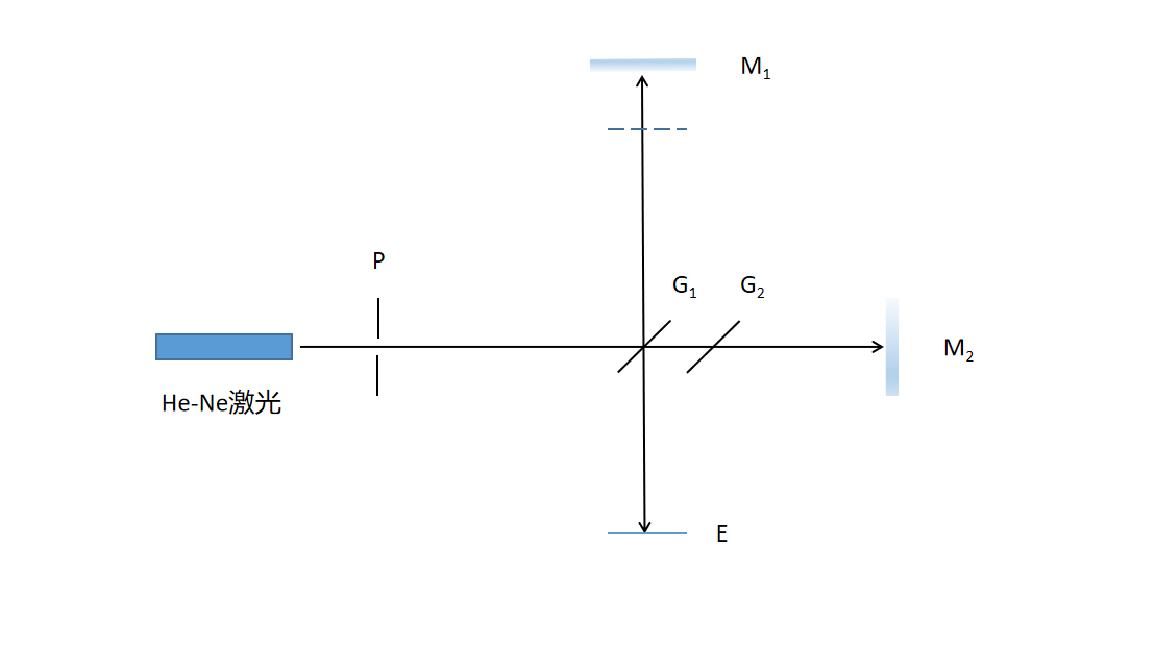
\includegraphics[width=.8\linewidth]{图片1.png}
		\caption{ 迈克尔逊干涉仪调节时的光路图}
	\end{figure}\noindent%
\end{enumerate}


\subsection{非定域干涉圆条纹和椭圆条纹的调节与变化规律及解释}
\subsubsection{非定域干涉圆条纹和椭圆条纹的调节}
\begin{enumerate}
	\item 在上面光路的基础上,把一短焦距的小透镜L加在光阑P和分束板$G_{1}$之间,并调节小透镜L,使得这个点光源均匀照射$M_{2}$。用观察屏E接收干涉条纹。此时,基本可以看到干涉条纹,但可能同心圆圆心不在E中央,调节$M_{2}$镜的微动螺丝,使得$M_{1}$和$M_{2}^{\prime}$相互平行,就可以观察到非定域的圆条纹,并且同心圆圆心基本在E中央。
	\item 将观察板E沿铅直轴转动,就可以观察到非定域的椭圆条纹。
\end{enumerate}
\subsubsection{非定域干涉圆条纹的变化规律及解释}
    将可移动的$M_{1}$镜大致调到90mm刻度处,然后不断向近处调节,观察到大致在90\~{}50mm时,条纹吞;大致在50\~{}30mm时,条纹吐。条纹的粗细变化如下表1。
    \begin{table}[H]
    	\centering\caption{非定域干涉圆条纹变化规律表}
    	\small
    	\begin{tabularx}{.85\linewidth}{C{1} *8{C{.5}}}
    		\toprule
    		\textbf{刻度/mm} &
    		90 &
    		60 &
    		55 &
    		50 &
    		45 &
    		40 &
    		30 & \\
    		\midrule
    		条纹粗细     & 细  & 较细 & 较粗 &  粗 & 较粗 & 较细  & 细 \\
    		条纹疏密     & 密  & 较密 & 较疏 &  疏 & 较疏 & 较密  & 密 \\
    		\bottomrule
    	\end{tabularx}
    	\vspace{3ex}
    \end{table}\noindent%

    由相干叠加公式可以得到观察板E上一点P的光强$$ I = I_{1} + I_{2} + 2*\sqrt{I_{1}* I_{2}}* \cos\delta$$
    因为初相位相同,相位差$\delta$有$$\delta = \frac{2*\pi}{\lambda}*(L_{2}- L_{1})$$
    从教材上给出的条件来计算,可以计算出$$L_{2}- L_{1} = 2d*(1-\frac{r^2}{2z^2})$$
    当$\delta = 2k\pi$时,光强最大,即出现亮条纹,可以得到等效条件	$$ L_{2}- L_{1} = k\lambda $$
    因为亮暗条纹都是等宽的,因此,条纹的宽窄和疏密可以一起讨论,相邻条纹可以有如下的计算
    $$ k\lambda = 2d*(1-\frac{r_{k}^2}{2z^2}) $$
    $$ (k-1)\lambda = 2d*(1-\frac{r_{k-1}^2}{2z^2}) $$
    $$ \lambda = d\dfrac{r_{k-1}^2 - r_{k}^2}{z^2} $$
    $$ r_{k-1} - r_{k} \approx \dfrac{\lambda * z^2}{2*d*r_{k}} $$
    通过这个式子,我们可以知道,越远离中心的条纹越密,越细;$M_{1}$和$M_{2}^{\prime}$之间距离d越大的条纹越细,越密。$M_{1}$镜大致在90\~{}50mm时,就是d减小;大致在50\~{}30mm时,就是d增大。
    条纹的吞吐可以有以下的计算
    $$ k_{1}\lambda = 2d*(1-\frac{r_{k_{1}}^2}{2z^2}) $$
    对于某一环来说,$M_{1}$和$M_{2}^{\prime}$之间距离d越大,则$k_{1}$增大,表现为条纹的吐;$M_{1}$和$M_{2}^{\prime}$之间距离d越小,则$k_{1}$减小,表现为条纹的吞。$M_{1}$镜大致在90\~{}50mm时,就是d减小;大致在50\~{}30mm时,就是d增大。


\subsection{非定域干涉直条纹和双曲条纹的调节}
\subsubsection{非定域干涉直条纹的调节}
在上面圆条纹的基础上,调节$M_{2}$镜后的微动螺丝,将同心圆圆心水平方向调出观察屏,并不断向该方向偏移,则在观察屏E上观察到的曲线曲率不断减小,逼近直线,最后在一定程度上可以认为调出了直线条纹。
\subsubsection{非定域干涉双曲条纹的调节}
在上面圆条纹的基础上,调节$M_{2}$镜后的微动螺丝,将同心圆圆心水平方向调出观察屏,并不断向该方向偏移,则在观察屏E上观察到的曲线曲率不断减小,当一定程度时,将观察板E沿铅直轴转动,就可以观察到非定域的双曲条纹。
	
\subsection{定域干涉等倾条纹的调节与变化规律及解释}
\subsubsection{定域干涉等倾条纹的调节}
将毛玻璃放在扩束透镜L和$ G_{1} $之间,在上面非定域干涉圆条纹粗而疏时,用眼睛代替观察屏E作为接收器,眼睛要聚焦到无穷远,此时可以观察到圆条纹,继续调节$M_{2}$镜后的微动螺丝,使得眼睛上下左右移动时,圆条纹的大小不变,并且也不吞吐,仅仅是圆心随眼睛移动。此时就是严格的等倾条纹了。
\subsubsection{定域干涉等倾条纹变化规律及解释}
 将可移动的$M_{1}$镜大致调到90mm刻度处,然后不断向近处调节,观察到大致在90\~{}50mm时,条纹吞;大致在50\~{}30mm时,条纹吐。条纹的粗细变化如下表2。
\begin{table}[H]
	\centering\caption{定域等倾干涉条纹变化规律表}
	\small
	\begin{tabularx}{.85\linewidth}{C{1} *8{C{.5}}}
		\toprule
		\textbf{刻度/mm} &
		90 &
		60 &
		55 &
		50 &
		45 &
		40 &
		30 & \\
		\midrule
		条纹粗细     & 细  & 较细 & 较粗 &  粗 & 较粗 & 较细  & 细 \\
		条纹疏密     & 密  & 较密 & 较疏 &  疏 & 较疏 & 较密  & 密 \\
		\bottomrule
	\end{tabularx}
	\vspace{3ex}
\end{table}\noindent%
因为初相位相同,相位差$\delta$有$$\delta = \frac{2*\pi}{\lambda}*(L_{2}- L_{1})$$
从教材上给出的条件来计算,可以计算出$$L_{2}- L_{1} = 2d*\cos\theta$$
当$\delta = 2k\pi$时,光强最大,即出现亮条纹,可以得到等效条件	$$ L_{2}- L_{1} = k\lambda $$
即$$ 2d*\cos\theta = k\lambda $$
因为中心条纹有$ \theta = 0 $,所以有关系
$$ 2d = k\lambda $$
对于中心来说,$M_{1}$和$M_{2}^{\prime}$之间距离d越大,则$k$增大,表现为条纹的吐;$M_{1}$和$M_{2}^{\prime}$之间距离d越小,则$k$减小,表现为条纹的吞。$M_{1}$镜大致在90\~{}50mm时,就是d减小;大致在50\~{}30mm时,就是d增大。\\
因为亮暗条纹都是等宽的,因此,条纹的宽窄和疏密可以一起讨论,相邻条纹可以有如下的计算
$$ 2d*\cos\theta_{k} = k\lambda $$
$$ 2d*\cos\theta_{k+1} = (k+1)\lambda $$
又因为$ \theta  $很小,所以有近似计算
$$ \theta_{k} - \theta_{k+1} \approx \dfrac{\lambda}{2d\theta_{k}} $$
通过这个式子,我们可以知道,越远离中心的条纹越密,越细;$M_{1}$和$M_{2}^{\prime}$之间距离d越大的条纹越细,越密。$M_{1}$镜大致在90\~{}50mm时,就是d减小;大致在50\~{}30mm时,就是d增大。

	
\subsection{定域干涉等厚条纹的调节与变化规律及解释}
\subsubsection{定域干涉等厚条纹的调节}
将毛玻璃放在扩束透镜L和$ G_{1} $之间,在上面非定域干涉圆条纹粗而疏时,用眼睛代替观察屏E作为接收器,眼睛要聚焦到无穷远,此时可以观察到圆条纹,继续调节$M_{2}$镜后的微动螺丝,使得$M_{1}$和$M_{2}^{\prime}$之间有很小的一夹角,调节$M_{1}$的位置,使得弯曲条纹往圆心方向移动。此时会出现定域干涉等厚直条纹。
\subsubsection{定域干涉等厚条纹变化规律及解释}
     将可移动的$M_{1}$镜大致调到90mm刻度处,然后不断向近处调节,观察到大致在90\~{}50mm时,条纹由弯曲变直;大致在50\~{}30mm时,条纹由直变弯曲。测量得到条纹最直时,即$M_{1}$和$M_{2}^{\prime}$左端相交时,$M_{1}$的刻度为$$ 50.71554 mm $$
     
     因为初相位相同,相位差$\delta$有$$\delta = \frac{2*\pi}{\lambda}*(L_{2}- L_{1})$$
     从教材上给出的条件来计算,可以计算出$$L_{2}- L_{1} = 2d*\cos\theta$$
     当$M_{1}$和$M_{2}^{\prime}$之间距离较小时,可以有近似$$ L_{2}- L_{1} = 2d $$
     即空气劈上厚度相同的位置,光程差相同,因此最后观察到的条纹曲率很小,可以看成直条纹。\\
     当$M_{1}$和$M_{2}^{\prime}$之间距离较大时,可以有近似$$ L_{2}- L_{1} = 2d*(1-\frac{\theta^2}{2}) $$
     即为了使同一干涉条纹上光程差相同,d必须增大,来抵消$\theta$增大引起的光程差减小。因此最后观察到的条纹曲率较大,是弯曲条纹。$M_{1}$镜大致在90\~{}50mm时,就是$M_{1}$和$M_{2}^{\prime}$之间距离减小;大致在50\~{}30mm时,就是$M_{1}$和$M_{2}^{\prime}$之间距离增大。
     

    
    
    



\section{压电陶瓷的压电常量的测量}
    压电陶瓷管长度L为46mm,壁厚t为1.0mm。调节迈克尔逊干涉仪,调出非定域干涉圆条纹,使用的是波长为632.8nm的激光。然后调节电压,数出吞吐的环数,记录下电压值和环数,测量得到下面数值
	\begin{table}[H]
		\centering\caption{测量电压值与圆条纹吞吐数的数据表}
		\small
		\begin{tabularx}{.85\linewidth}{C{1} *5{C{.8}}}
			\toprule
			\textbf{吞吐环数N} &
			0 &
			1 &
			2 &
			3 & \\
			\midrule
			电压值$ U_{f} $/V     & 100  & 62.6 & 34.2 &  18.8    \\
			\bottomrule
		\end{tabularx}
		\vspace{3ex}
	\end{table}\noindent%
    压电常量定义有
    $$ \dfrac{\Delta L}{L} = d_{21} * E $$
    又因为
    $$ 2 * \Delta L = N * \lambda $$
    因此有
    $$ N = \frac{2}{\lambda} * \frac{L}{t} *d_{21} * U_{f} $$
    利用线性回归可以得到
    $$ a = - 0.0356 $$
	$$ b = 3.42$$
	$$ r = -0.984 $$
	因此又有
	$$ a = \frac{2}{\lambda} * \frac{L}{t} *d_{21} $$
	$$ d_{21} = 0.245 nm/V $$
	
	


\section{分析与讨论}
\subsection{分析实验中测量压电常量的误差}
    计算不确定度有
    $$ \dfrac{\sigma_{d_{21}}}{d_{21}} = \dfrac{\sigma_{a}}{a} $$
    $$ \dfrac{\sigma_{a}}{a} = \sqrt{\dfrac{\frac{1}{r^2} - 1}{n-2}} = \dfrac{\sigma_{d_{21}}}{d_{21}} $$
    所以有
    $$ \sigma_{d_{21}} = 0.031 $$
    $$ d_{21} \pm \sigma_{d_{21}} = 0.245 \pm 0.031 nm/V $$
    
    实验中还有一些其他的无法计算的误差,比如对于环的吞吐的判断界限比较主观,这往往会带来一定的误差。
    

	

	
\subsection{分析实验中交棱时$M_1$刻度的误差}
    $M_1$刻度l的不确定度关系有
	$$ \sigma_l = \dfrac{e}{\sqrt{3}}$$
	$$ e = 0.00005$$
	因此可以计算
	$$ \sigma_l = 0.00003 mm $$
	$$ l \pm \sigma_{l} = 50.71554 \pm 0.00003 mm$$
	实验中还有一些其他的无法计算的误差,比如对于条纹在何时最直的判断比较主观,这往往会带来一定的误差。
	



	
\section{收获与感想}
\begin{enumerate}
	\item 在做光学实验时,光路的校准是一个非常重要的内容。在校准的过程之中一定要遵守先校准的元件就不可以再次调节的原则,依次按顺序校准。这就要求在试验方案的设计上充分考虑每个光学元件的特性与校准的难易程度,设计出合理的校准方案。
	\item 激光束不能直接射入人眼,会造成危险。
	\item 迈克尔逊干涉仪是精密仪器,在旋转和调整螺丝和手轮是要轻,动作要稳,不能用手触摸镜片,不要冲着仪器说话、咳嗽。
	\item 同方向调节粗转鼓轮和微调鼓轮可以消除回程差;若调节过程中有反向转动,则需要重新调节,以消除回程差。
\end{enumerate}



	\vfill\noindent\itshape\footnotesize
	\hfill Last edited: \today\ \copyright\ 赵启渊
\end{document}